\documentclass[main.tex]{subfiles}
\begin{document}
虎克固体与牛顿流体的本构关系不足以描述聚合物流体的流变学性质。聚合物流体是一种复杂流体(complex fluid),即具有粘弹性(viscoelasticity)和非线性(nonlinearity)的流体。

虎克固体和牛顿流体的本构关系的“简单”之处在于:
\begin{enumerate}
    \item 应力只与应变或应变的时间导数有关
    \item 应力与应变或应变的时间导数的关系是线性的\footnote{线性(linearity)是指,对于一个系统,如果输入\(x_1\left(t\right)\)和\(x_2\left(t\right)\)的输出是\(y_1\left(t\right)\)和\(y_2\left(t\right)\),则输入\(k_1x_1\left(t\right)+k_2x_2\left(t\right)\)的输出就是\(k_1y_1\left(t\right)+k_2y_2\left(t\right)\)的性质。虎克固体和牛顿流体的本构关系满足此性质。\authornumcite{何曼君2007}\S 8.4中所介绍的元件模型均有此性质,可自行验证。}。
\end{enumerate}
复杂流体的“复杂”之处分别是对上述两条理想情况的偏离:
\begin{enumerate}
    \item 本构关系中包括应力、应力的时间导数、应变、应变的时间导数这四类函数中的三类或三类以上的函数\footnote{读者可自行验证,\authornumcite{何曼君2007}\S 8.5中的各种元件模型的方程均满足这一描述。};
    \item 物料函数依赖应变、应力或它们的时间导数;或者说应力与应变名应变的时间导数的关系是非线性的。
\end{enumerate}
第一种复杂性就是粘弹性,第二种复杂性就是非线性。理论上一个复杂流体可以只满足这两种复杂性质的其中一种。但真实的复杂流体常常同时具有两种复杂性质,即非线性粘弹性(nonlinear viscoelasticity)。

复杂流体的这两方面复杂性还可以更粗略的说成:复杂流体的流变学行为依赖外场的作用时间(粘弹性)和作用强度(非线性)。这一表述更符合我们的直观印象。

\begin{figure}[h]
\centering
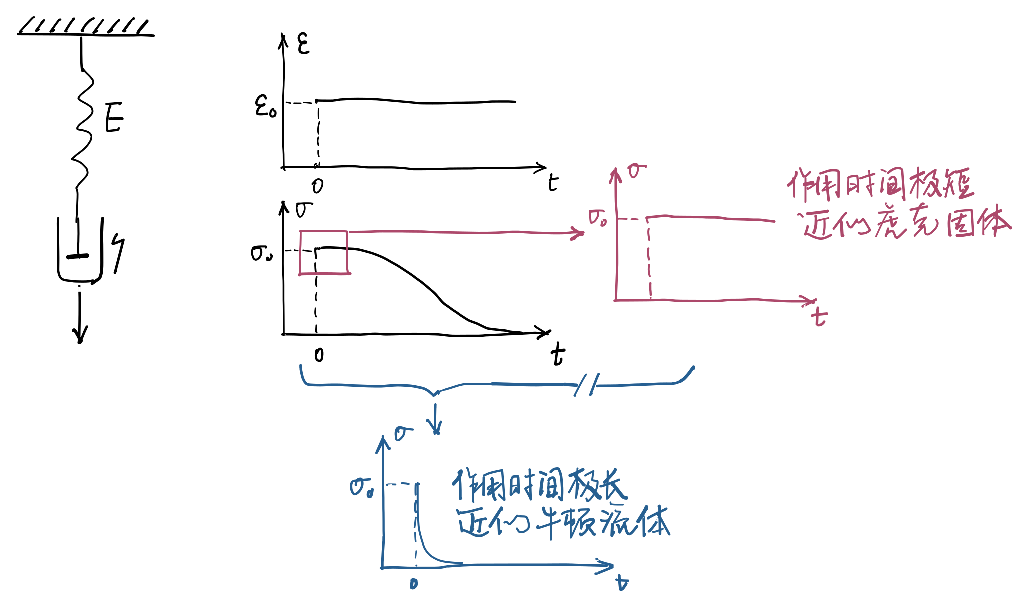
\includegraphics[width=0.5\textwidth]{images/I.2.1.eps}
\caption{Maxwell模型的应力松弛实验}
\label{fig:I.2.1}
\end{figure}

\begin{example}[应力松弛实验]
Maxwell模型的标量本构关系\cite[\S8.5.1,p.~240]{何曼君2007}:
\[\sigma\left(t\right)=\frac{\eta}{\tau}e^{-\frac{t}{\tau}}\]
测试结果如图\ref{fig:I.2.1}所示。当应变时间极短时,模型的响应近似虎克固体;当应变时间极长时,模型的响应近似牛顿流体。可定义Deborah数$De\equiv\tau/t$,当$De\rightarrow0$时材料呈液体响应;当$De\rightarrow\infty$时材料呈固体响应。
\end{example}

\begin{figure}[h]
\centering
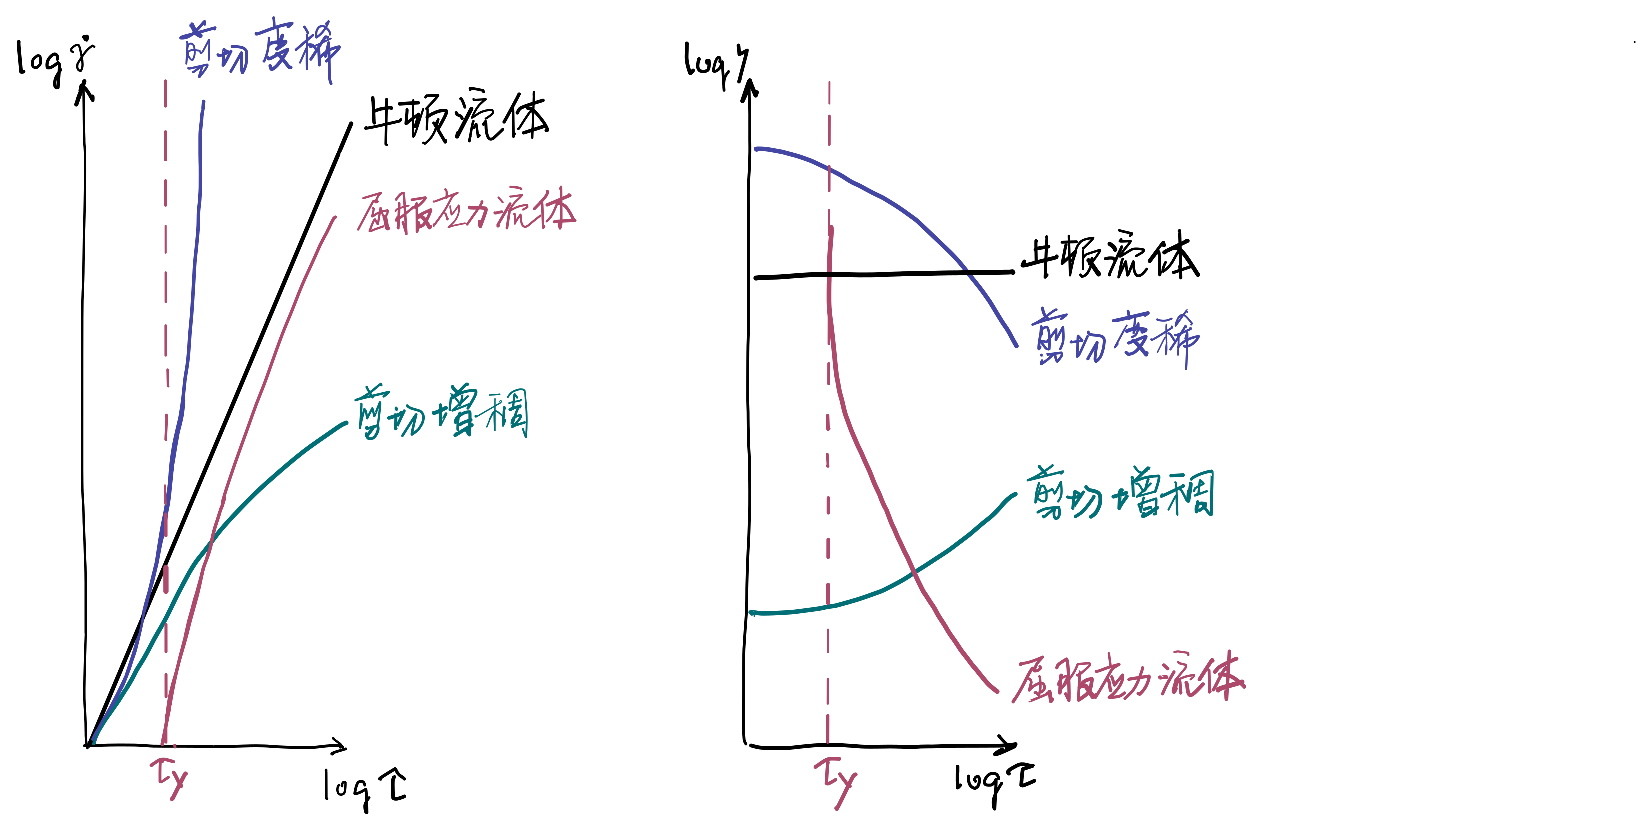
\includegraphics[width=0.5\textwidth]{images/I.2.2.eps}
\caption{非牛顿流体的流动曲线}
\label{fig:I.2.2}
\end{figure}

\begin{example}
各类非牛顿流体在如例\ref{exp:I.1.3}中的简单剪切下的定常流动规律如图\ref{fig:I.2.2}所示:剪切变稀(shear-thinning),剪切增稠(shear-thickening),屈服应力流体(yield-stress fluid)。
\end{example}

非线性粘弹性——Weissenberg效应(爬杆效应):Weissenberg数$Wi\equiv\tau\dot{\gamma}=\tau\frac{\gamma}{t}=De\gamma$。

非线性粘弹性——触变性(thixotropy):屈服应力流体的屈服流动与恢复明显依赖时间的性质。

流变学主要研究复杂流体的非线性粘弹性本构关系。
\end{document}